%\documentclass[yellow,mathserif,handout]{beamer}
\documentclass[xcolor=pdftex,table,10pt,yellow,mathserif]{beamer}
\usepackage[3D]{movie15}
\usepackage{array}
\usepackage{amsmath}
\usepackage{tikz}
\usepackage{pgflibraryshapes}  




\usepackage[english]{babel}
\usepackage[latin1]{inputenc}
\usepackage{times}
%\usepackage[T1]{fontenc}
%\usepackage{color}
%\usepackage[x11names, rgb]{xcolor}
\usepackage{listings}
\usepackage{colortbl}
%\usepackage{dot2texi}
\usepackage{verbatim}
%\usepackage{pgfplots}
%\usetikzlibrary{arrows,shapes,backgrounds,snakes}
\usetikzlibrary{arrows}
%\usefonttheme{professionalfonts}
\usefonttheme[onlymath]{serif}







%\usetheme{PSI}
\usetheme{Madrid}

\usepackage[overlay,absolute]{textpos}
\TPGrid[4mm,25mm]{10}{5}


\newcommand{\opal}{\textsc{OPAL }}
\newcommand{\opalt}{\textsc{OPAL-t }}
\newcommand{\opalcycl}{\textsc{OPAL-cycl }}
\newcommand{\opalmap}{\textsc{OPAL-map }}

\newcommand{\mad}{\textsc{mad }}
\newcommand{\madnine}{\textsc{mad9 }}
\newcommand{\madninep}{\textsc{mad9p }}
\newcommand{\madeight}{\textsc{mad8 }}
\newcommand{\pooma}{\textsc{pooma }}
\newcommand{\classic}{\textsc{classic }}
\newcommand{\hfifepart}{\textsc{H5Part }}
\newcommand{\hfifefe}{\textsc{H5FE }}

\renewcommand{\epsilon}{\varepsilon} 
\renewcommand{\vec}[1]{{\bf #1}} 
\newcommand{\dt}[1]{\frac{\partial #1}{\partial t}}
\newcommand{\dtt}[1]{\frac{\partial^2 #1}{\partial t^2}}
\newcommand{\dtvec}[1]{\frac{\partial {\mathbf #1}}{\partial t}}
\newcommand{\dttvec}[1]{\frac{\partial^2 {\mathbf #1}}{\partial t^2}}
\newcommand{\rot}{\vec{\nabla} \wedge }
\renewcommand{\div}{\vec{\nabla} \cdot }
\newcommand{\bs}[1]{\mathbf #1}
\newcommand{\mc}[1]{\mathcal #1}

\def\vec#1{\mathbf{#1}}
\def\vecg#1{\boldsymbol{#1}}
\def\norm#1{\| #1 \|} 
\def\tr{^{\!\top}}
%\def\curl{\nabla\times}
%\def\div{\nabla\cdot}
\def\curl{{\bf curl}\,}
\def\curlp{{\rm curl}_p\,}
\def\div{{\rm div}\,}
\def\grad{\nabla}
\def\gradp{\nabla_p}
\def\dotp#1#2{\langle#1,#2\rangle}
\def\eps{\varepsilon}

\newcommand{\mat}[1]{\ensuremath{\boldsymbol{#1}}}
\newcommand{\vect}[1]{\ensuremath{\mathbf{#1}}}
\newcommand{\iprod}[2]{\ensuremath{\langle#1,#2\rangle}}
\newcommand{\abs}[1]{\ensuremath{|#1|}}
\newcommand{\Nedelec}{N\'{e}d\'{e}lec}

\newcommand{\id}[1]{\structure{#1}}

\renewcommand {\Re}{{\mathbb{R}}}
\newcommand {\Co}{{\mathbb{C}}}
\newcommand {\Int}{{\mathbb{Z}}}
\newcommand {\Nat}{{\mathbb{N}}}
%%
%%
\newcommand {\Hcurl}{{H(\mathbf{curl};\Omega)}}
\newcommand {\Hocurl}{{H_0(\mathbf{curl};\Omega)}}
\newcommand {\Hdiv}{{H(\mathrm{div};\Omega)}}
\newcommand {\Hodiv}{{H_0(\mathbf{div};\Omega)}}
%%
\renewcommand {\Re}{{\rm I \kern-2pt R}}
\newcommand{\vc}[1]{\mbox{\boldmath $#1$}}



\mode<presentation>
{

  \usepackage{pgf}
  \usepackage{hyperref}

% \usetheme{PSI}
 %\useinnertheme{PSI} 
   \setbeamercovered{transparent}
  \setbeamercovered{transparent}  
}

\setbeamertemplate{footline}
{
	\leavevmode%
	\hbox{%
%	\begin{beamercolorbox}[wd=.14\paperwidth,ht=2.25ex,dp=1ex,center]{author in head/foot}%
%		\usebeamerfont{author in head/foot}\insertshortauthor
%	\end{beamercolorbox}%
%	\begin{beamercolorbox}[wd=.48\paperwidth,ht=2.25ex,dp=1ex,center]{title	in head/foot}%
%		\usebeamerfont{title in head/foot}\insertshorttitle
%	\end{beamercolorbox}%
	\begin{beamercolorbox}[wd=1.\paperwidth,ht=2.25ex,dp=1ex,right]{date in head/foot}%
		\usebeamerfont{date in head/foot}\insertshortdate{}\hspace*{2em}
		\insertframenumber{} /
		\inserttotalframenumber\hspace*{2ex} 
	\end{beamercolorbox}}%
	\vskip0pt%
}


\setbeamertemplate{navigation symbols}{}


\usepackage[latin1]{inputenc}
\usepackage[english]{babel}

\title{Introduction to OPAL - Part 1} 

\author{Andreas Adelmann, K. Kraus, Y. Ineichen (ETH), \\J. Yang (Tsinghua Univ., China \& CIAE)}
\date{\today}

\begin{document}

\frame{
\maketitle


\begin{center}

  
\includegraphics{figures/psi_logo_narrow} 
      \end{center}

}

\begin{frame}
	  \frametitle{Outline}
	  \tableofcontents
	\end{frame}


\section{OPAL in a Nutshell}

\begin{frame}{OPAL in a Nutshell} 
\begin{alertblock}{}  
 \opal is a tool for charged-particle optics in
accelerator structures and beam lines.  The main focus is on 3D modelling in large structures.
\end{alertblock}
\begin{block}{}  
\begin{itemize}
\item \opal is derived from \madninep and is based 
on the
\htmladdnormallink{CLASSIC}{http://wwwslap.cern.ch/classic/} class library.

\item Independent Parallel Particle Layer (IPPL) is
the framework which provides parallel particles and fields using data parallel ansatz. 

\item \opal is build from ground up
as a parallel application having in mind that: High Performance Computing (HPC) is the third leg of 
science, which complements theory and the experiment. 
\item  \opal runs on your laptop as well as on the largest HPC clusters. 
\item \opal uses the \mad language with extensions.
\item \opal (and all other used frameworks) are written in C++ using OO-techniques, hence \opal is very easy to extend.
\item Documentation is taken very serious at both levels: source code and user manual. Checkout: \url{ http://amas.web.psi.ch/docs/index.html}.
\end{itemize}
\end{block}
\end{frame}

\section{\opal Flavours}
\begin{frame}{\opal Flavours}
\begin{block}{}  
The following OPAL flavours  exist:
\begin{itemize}
\item \opalt 
\begin{itemize}
\item \opalt   tracks particles which 3D space charge uses time as the independent variable, and can be used to model guns, injectors and complete XFEL's but without the undulator.
\end{itemize}
\item \opalcycl 
\begin{itemize}
\item \opalcycl tracks particles which 3D space charge including neighbouring turns in cyclotrons
with time as the independent variable. 
\end{itemize}
\item \opalmap (not yet released)
\begin{itemize}
\item \opalmap tracks particles with 3D space charge using split operator techniques, and is a proper subset of \madninep. %In the future there will be also a linear space charge mode available which allows one to track moments of the distribution. 
\end{itemize}
\end{itemize}
\end{block}
%\begin{block}{Lorentz Force Equation}  
%  \begin{columns}
%    \begin{column}{3.5cm}
%      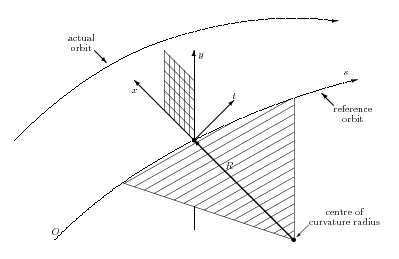
\includegraphics[width=0.8\linewidth]{figures/localcs.png}
%    \end{column}
%    \begin{column}{8cm}
%  \begin{block}{} \footnotesize
%  With $m_0$ the rest mass, $\gamma = (1-\beta^2)^{-1/2}$ and $\vc{\beta} =
%\frac{\vc{v}}{c}$ 
%\begin{align*}
%     \dot{\vc{p}} = \vc{F}(\vc{v},\vc{x},t) = Q\;(\vc{v} \times \vc{B} + \vc{E})
% \end{align*} 
% In general all quantities are time and position dependent.
%\end{block}
%\end{column}
%\end{columns}
%\end{block}

\end{frame}



\begin{frame}[fragile]
\frametitle{\opal Flavours} 
\framesubtitle{Sketch of an inputfile - \opalt}
\begin{block}{}
\begin{verbatim}
TITLE,STRING="OPAL XFEL 30 MeV Diagnostics section";
Edes=0.0307;      // GeV
gamma=(Edes+EMASS)/EMASS;

FINLB02_MSLAC40: SOLENOID, L=0.001, KS=0.05, 
FMAPFN="FINLB02-MSLAC.T7", ELEMEDGE=4.554;

FIND1_MQ10: QUADRUPOLE, L=0.1, K1=2.788, ELEMEDGE=5.874;

FIND1:   LINE = (FINLB02_MSLAC40, FIND1_MQ10 ...);

Dist1:DISTRIBUTION, DISTRIBUTION=GAUSS,
SIGMAX=  1.0e-03, SIGMAPX=1.0e-4, CORRX=0.5,
SIGMAY=  2.0e-03, SIGMAPY=1.0e-4, CORRY=-0.5,
SIGMAT=  3.0e-03, SIGMAPT=1.0e-4, CORRT=0.0;
\end{verbatim}
\end{block}
\end{frame}


\begin{frame}[fragile]
\frametitle{\opal Flavours} 
\framesubtitle{Sketch of an inputfile - \opalt cont.}
\begin{block}{}
\begin{verbatim}
Fs2:FIELDSOLVER, FSTYPE=FFT, MX=32, MY=32, MT=64, 
        PARFFTX=false, PARFFTY=false, PARFFTT=true,
        BCFFTX=open, BCFFTY=open, BCFFTT=open,
        BBOXINCR=1.0, GREENSF=INTEGRATED;

beam1: BEAM, PARTICLE=ELECTRON, PC=P0, NPART=1e5, 
BFREQ=1498.953425154e6, BCURRENT=0.299598, CHARGE=-1;

SELECT, LINE=FIND1;

TRACK,LINE=FIND1, BEAM=beam1, MAXSTEPS=10000, DT=1.0e-12;
 RUN, METHOD = "PARALLEL-T", BEAM=beam1, 
 FIELDSOLVER=Fs2, DISTRIBUTION=Dist1;
endtrack;
Stop;
\end{verbatim}
\end{block}
\end{frame}




%%%%%%%%%%%%%%%%%%%%%%%%%%%%%%%%%%%%%%%%%%%%%%%%%%%%%%%%%%%%%%%%%%%%%%%%%%%%%%%%
\begin{frame}{\opal Flavours} {PIC $\rightarrow$ Maxwell's Equation in the Electrostatic approximation}
   \begin{center}
     \begin{tikzpicture}
       \begin{scope}[shape=rectangle,rounded corners,fill=yellow!40,text centered]
         \node[shape=circle,fill=yellow!40, text width=2cm] (magopt) at (-3,0) {Magnetic Optics};
         \node[shape=circle,fill=blue!40, text width=2cm] (mpd) at (3,0) {N-Body Dynamics};
         \node[fill=yellow!40,text width=3.6cm,minimum height=1.8cm] at (-2,2.0) {\vspace{-\abovedisplayskip}\begin{gather*}\curl \mat{E} + \frac{\partial\mat{B}}{\partial t} = 0 \\ \div \mat{B} = 0\end{gather*}\vspace{-2\belowdisplayskip}};
         \node[fill=blue!40,text width=3.6cm,minimum height=1.8cm] at (2,2.0) {$\div \mat{E} = \rho/\eps_0$};
         \node (h) at (0,0) {$\mat{H} = \mat{H}_\text{ext} + \mat{H}_\text{sc}$};
         \node (formM) at (0,-2) {};
         \node[fill=red!40] at (0,-2.0) {${\cal M}(s) = {\cal M}_\text{ext}(s/2) \otimes {\cal M}_\text{sc}(s) \otimes {\cal M}_\text{ext}(s/2) + { \cal O}(s^3)$};
         \node[fill=red!40] at (0,-3.0) {RK-4 and the implicit $D_1$ scheme \footnote{\tiny Birdsall \& Langdon "Plasma Physics via Computer Simulation}};
       \end{scope}
       \node[draw,text width=2.5cm,text centered] at (-4.5,1.2) {\bf Lie Algebraic Methods};
       \node[draw,text width=2.5cm,text centered] at (4.5,1.2) {\bf 3D Poisson Solver};
     \end{tikzpicture}
   \end{center}
%   When using time integration: RK4 and $D_1$ algorithm from Birdsall and Langdon's book (ada need more)
 \end{frame}

\section{Architecture}
\begin{frame}{Architecture}
 \begin{tikzpicture}
    \footnotesize
     \node[shape=rectangle,rounded corners,minimum width=11.0cm,minimum height=5.0cm,fill=green] at (3.125,-1) {};
      \begin{scope}[shape=rectangle,rounded corners,minimum width=3.0cm,minimum height=0.7cm,fill=yellow,text centered]
      \node[fill= green] (0_00) at (0,1.0) {Solvers: Direct,MG};
      \node[fill= green] (0_00) at (3.5,1.0) {Integrators};
      \node[fill= green] (0_00) at (7.0,1.0) {Distributions};
       \node[fill= red] (q_00) at (0,0) {FFT};
       \node[fill= red] (q_01) at (3.5,0) {D-Operators};
       \node[fill= red] (q_02) at (7,0) {NGP,CIC, TSI};
       \node[fill= red] (q_10) at (0,-0.75) {Fields};
       \node[fill= red] (q_11) at (3.5,-0.75) {Mesh};
       \node[fill= red] (q_12) at (7,-0.75) {Particles};
       \node[fill=red] (q_20) at (0,-1.5) {Load Balancing};
       \node[fill=red] (q_21) at (3.5,-1.5) {Domain Decomp.};
       \node[fill=red] (q_22) at (7,-1.5) {Message Passing};
       \node[fill=red] (q_20) at (0,-2.25) {STL};
       \node[fill=red] (q_21) at (3.5,-2.25) {PETE};
       \node[fill=red] (q_22) at (7,-2.25) {Polymorphism};
       \node[rotate=90,minimum width=4.75cm,fill=blue] (bla) at (-1.9,-1) {\classic};
%        \node[fill=magenta,minimum width=7.0cm] (q_23) at (2.0,-3.0) {\hfifepart};
      \end{scope}
% \draw (q_A) -- (q_1) -- (q_2) -| (q_E);
   %  \draw[->,shorten >=2pt] (q_A) .. controls +(75:1.4cm) and +(105:1.4cm) .. node[above] {$x$} (q_A);
 \end{tikzpicture}  
 \vspace{-0cm}
   \begin{itemize}
   \item {\bf\color{green}  \opal Object Oriented Parallel Accelerator Library}
   \item {\color{red} $\text{IP}^{2}L$ Independent Parallel Particle Layer}
   \item {\color{blue} \classic Class Library for Accelerator Simulation System and Control}
 %  \item  {\bf\color{magenta} \hfifepart for parallel particle and structured field I/O (HDF5) }
  \end{itemize}
 \end{frame}
 
 
 \begin{frame}
\frametitle{Architecture}
\framesubtitle{Connection with other Frameworks}
\vspace{-1cm}
\begin{center}
\tikzstyle{format} = [draw, thin, fill=blue!20]
\tikzstyle{pblock} = [rectangle, draw, fill=blue!20, text width=6em, text centered, rounded corners, minimum height=0.4em]
\tikzstyle{mblock} = [rectangle, draw, fill=green!20, text width=6em, text centered, rounded corners, minimum height=0.4em]
\tikzstyle{bblock} = [rectangle, draw, fill=gray!20, text width=6em, text centered, rounded corners, minimum height=0.4em]
\tikzstyle{prblock} = [rectangle, draw, fill=red!20, text width=6em, text centered, rounded corners, minimum height=0.4em]
\tikzstyle{rblock} = [rectangle, draw, fill=olive!20, text width=6em, text centered, rounded corners, minimum height=0.4em]
%\tikzstyle{block} = [rectangle, draw, fill=blue!20, text centered, rounded corners]
\tikzstyle{decision} = [diamond, draw, fill=blue!20, text width=4.5em, text badly centered, node distance=3cm, inner sep=0pt]
\tikzstyle{medium} = [ellipse, draw, thin, fill=green!20, minimum height=2.5em]
\tikzstyle{cloud} = [draw, ellipse,fill=red!20, node distance=3cm, minimum height=2em]
\tikzstyle{line} = [draw, -latex']
\tikzstyle{emptyblock} = [rectangle]


\begin{tikzpicture}[scale=0.8,transform shape,node distance=3cm]%[node distance = 3cm, scale=0.5]
    % Place nodes
    \node [pblock] (STEP) {
		     STEP file};
    \node [bblock, right of=STEP] (BOGUI) {
		     heronion};
    \node [mblock, right of=BOGUI] (surfmesh) {
		     surface mesh};
    \node [mblock, below of=surfmesh] (add) {
		     mesh, ...};
    \node [pblock, right of=surfmesh] (H5FED) {
		     H5FED};
    \node [pblock, above of=H5FED] (H5Part) {
		     H5Part};

    \node [pblock, below of=H5FED] (VTK) {
    		     VTK};
    \node [bblock, right of=H5FED] (OPAL) {
    		     OPAL};
		  
    % Draw edges
    \path [line] (STEP) -> (BOGUI);
    \path [line] (BOGUI) -> (surfmesh);
    \path [line,style=dashed, ->] (BOGUI) edge [out=-90, in=90] (add);
    \path [line] (surfmesh) -> (H5FED);
    \path [line,style=dashed, ->] (surfmesh) edge [out=-90, in=90] (VTK);
    %\path [->] (fifth) edge [out=-90, in=90] (distmesh);
    \path [->] (H5FED) edge (OPAL);
    \path [line,style=dashed, ->] (H5FED) edge [out=90, in=180] node[right] {part of} (H5Part);
    \path [<->] (H5Part) edge [out=0, in=90] (OPAL);
    

\end{tikzpicture}

%\begin{tikzpicture}[overlay]
%	\path[->]<1-> (third) (fifth);
%	\path[->,red!40,thick]<2-> (second) edge [bend right] (fifth);
%\end{tikzpicture}

\end{center}
\small{in collaboration with B. Oswald, T. Schietinger and A. Gsell (AIT)}
\end{frame}
 
 \section{Parallel Issues}
\begin{frame}{Parallel Issues}{\opal Scaling on Cray XT3  "Horizon" at CSCS}
  \begin{columns}
    \begin{column}{4.5cm}
      \scriptsize
      \begin{block}{Production Run Setup}
        \begin{itemize}
        \item Tracking $10^7$ particles 
        \item 3D FFT on a $256^3$ grid
        \item Gaussian distribution
        \item no parallel I/O
        \end{itemize}
      \end{block}
      \end{column}
      \begin{column}{6.5cm}
      \begin{block}{Observations}
        \begin{itemize}
        \item Solver scales still well
        \item Load balancing not optimal anymore 
        \item Moving mesh has a problem 
        \end{itemize}
     \end{block}
    \end{column}
  \end{columns}
  \vspace{-.8cm}
      \begin{center}
      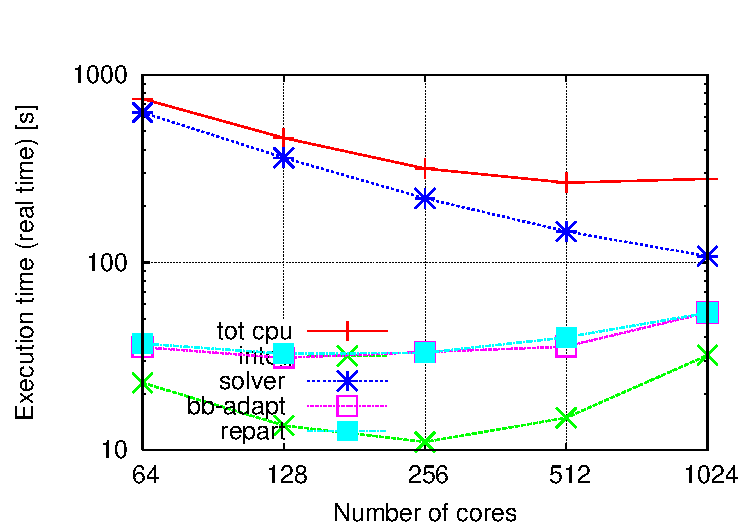
\includegraphics[scale=0.45]{figures/timing-mult-1-PPP-large}    % PPS timing-mult-1-1small1}
        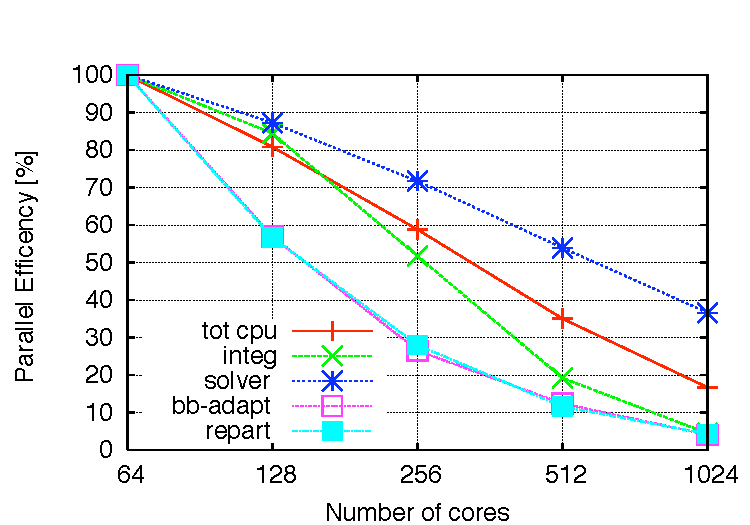
\includegraphics[scale=0.45]{figures/timing-mult-2-PPP-large}  % PPS timing-mult-1-2small2}
      \end{center}
\end{frame}

\begin{frame}{Parallel Issues}{$\text{IP}^{2}L$ FFT Kernel Scaling}
  \begin{columns}
    \begin{column}{10.cm}
      \begin{block}{}
        \begin{itemize}
    % \item Solver Kernel i.e. FFT \& Fieldinterpolation 
        \item 3D FFT ($G_1=2048^3$, $G_2=4096^3$) 
        \item 2D domain decomposition, $P= 512 \dots 4096$\footnote{obtained on Franklin (Cray XT4 at LBNL) number 5 on the Top-500}
           \item \alert{Kernel scales very well} 
        \end{itemize}
      \end{block}
      \end{column}
  \end{columns}
  \vspace{-.3cm}
      \begin{center}
      \includegraphics[scale=0.25]{figures/fft2-1-Franklin}    % PPS timing-mult-1-1small1}
      \end{center}
\end{frame}

\begin{frame}{Parallel Issues}{Reality or Fiction?}
\vspace{-0.2cm}
\begin{block}{}
Your Laptop would be at the bottom of the Top-500 list around 1997-98!
\end{block}
\vspace{-1cm}
   \begin{center}
      \includegraphics[scale=0.25]{figures/hans-proj}    
      \end{center}
  \vspace{-1.5cm}    
\begin{block}{}
Our FELSI-cluster would be number one of the Top-500 list in 1997!
\end{block}      
\begin{block}{Implications}
Using the technology ahead will enable us to speedup computations while increasing the accuracy of the used models. We can enter into
new regimes of accelerator modelling and controls.  
\end{block}     
\end{frame}


\section{\opal V 1.1.0 Release \& Roadmap of new Features}

\begin{frame}{\opal V 1.1.0 Release \& Roadmap of new Features}

\begin{block}{}
\begin{table}[ht]\footnotesize
\begin{center}
\begin{tabular}{p{7cm}c}
\hline
{\bf Name} & {\bf Version (estimated)} \\
\hline
{\bf Algorithms} & \\
ML based space charge solver & 1.1.1 \\
1D csr wake fields & 1.1.1 \\
Bet/HOMDYN Model (Envelope Solver) & end of summer 1.1.3\\
longitudinal and transverse short range wake fields& end of summer 1.1.3 \\
3D(2D) FETD self-consistent solver & 1.x \\
\opalmap & 1.x \\
\hline
{\bf New Elements} &  \\
SBend & 1.1.0 \\
Quadrupole & 1.1.0 \\
Screen & 1.1.0 \\
Collimator & 1.1.1 \\
Multipole & 1.1.x \\
\hline
\end{tabular}
\caption{List of features which will be implemented in versions to come (please note: the estimated version numbers are non-binding).}
\label{roadmap}
\end{center}
\end{table}
\end{block}
\end{frame}

\end{document}

